\documentclass[11pt,compress,t,notes=noshow, xcolor=table]{beamer}

\documentclass[11pt,compress,t,notes=noshow, xcolor=table]{beamer}
\usepackage[]{graphicx}\usepackage[]{color}
% maxwidth is the original width if it is less than linewidth
% otherwise use linewidth (to make sure the graphics do not exceed the margin)
\makeatletter
\def\maxwidth{ %
  \ifdim\Gin@nat@width>\linewidth
    \linewidth
  \else
    \Gin@nat@width
  \fi
}
\makeatother

\definecolor{fgcolor}{rgb}{0.345, 0.345, 0.345}
\newcommand{\hlnum}[1]{\textcolor[rgb]{0.686,0.059,0.569}{#1}}%
\newcommand{\hlstr}[1]{\textcolor[rgb]{0.192,0.494,0.8}{#1}}%
\newcommand{\hlcom}[1]{\textcolor[rgb]{0.678,0.584,0.686}{\textit{#1}}}%
\newcommand{\hlopt}[1]{\textcolor[rgb]{0,0,0}{#1}}%
\newcommand{\hlstd}[1]{\textcolor[rgb]{0.345,0.345,0.345}{#1}}%
\newcommand{\hlkwa}[1]{\textcolor[rgb]{0.161,0.373,0.58}{\textbf{#1}}}%
\newcommand{\hlkwb}[1]{\textcolor[rgb]{0.69,0.353,0.396}{#1}}%
\newcommand{\hlkwc}[1]{\textcolor[rgb]{0.333,0.667,0.333}{#1}}%
\newcommand{\hlkwd}[1]{\textcolor[rgb]{0.737,0.353,0.396}{\textbf{#1}}}%
\let\hlipl\hlkwb

\usepackage{framed}
\makeatletter
\newenvironment{kframe}{%
 \def\at@end@of@kframe{}%
 \ifinner\ifhmode%
  \def\at@end@of@kframe{\end{minipage}}%
  \begin{minipage}{\columnwidth}%
 \fi\fi%
 \def\FrameCommand##1{\hskip\@totalleftmargin \hskip-\fboxsep
 \colorbox{shadecolor}{##1}\hskip-\fboxsep
     % There is no \\@totalrightmargin, so:
     \hskip-\linewidth \hskip-\@totalleftmargin \hskip\columnwidth}%
 \MakeFramed {\advance\hsize-\width
   \@totalleftmargin\z@ \linewidth\hsize
   \@setminipage}}%
 {\par\unskip\endMakeFramed%
 \at@end@of@kframe}
\makeatother

\definecolor{shadecolor}{rgb}{.97, .97, .97}
\definecolor{messagecolor}{rgb}{0, 0, 0}
\definecolor{warningcolor}{rgb}{1, 0, 1}
\definecolor{errorcolor}{rgb}{1, 0, 0}
\newenvironment{knitrout}{}{} % an empty environment to be redefined in TeX

\usepackage{alltt}
\newcommand{\SweaveOpts}[1]{}  % do not interfere with LaTeX
\newcommand{\SweaveInput}[1]{} % because they are not real TeX commands
\newcommand{\Sexpr}[1]{}       % will only be parsed by R
\newcommand{\xmark}{\ding{55}}%


\usepackage[english]{babel}
\usepackage[utf8]{inputenc}

\usepackage{dsfont}
\usepackage{verbatim}
\usepackage{amsmath}
\usepackage{amsfonts}
\usepackage{amssymb}
\usepackage{bm}
\usepackage{csquotes}
\usepackage{multirow}
\usepackage{longtable}
\usepackage{booktabs}
\usepackage{enumerate}
\usepackage[absolute,overlay]{textpos}
\usepackage{psfrag}
\usepackage{algorithm}
\usepackage{algpseudocode}
\usepackage{eqnarray}
\usepackage{arydshln}
\usepackage{tabularx}
\usepackage{placeins}
\usepackage{tikz}
\usepackage{setspace}
\usepackage{colortbl}
\usepackage{mathtools}
\usepackage{wrapfig}
\usepackage{bm}
\usepackage{amsmath}
\usepackage{pifont}

\usetikzlibrary{shapes,arrows,automata,positioning,calc,chains,trees, shadows}
\tikzset{
  %Define standard arrow tip
  >=stealth',
  %Define style for boxes
  punkt/.style={
    rectangle,
    rounded corners,
    draw=black, very thick,
    text width=6.5em,
    minimum height=2em,
    text centered},
  % Define arrow style
  pil/.style={
    ->,
    thick,
    shorten <=2pt,
    shorten >=2pt,}
}

\usepackage{subfig}

% Defines macros and environments
\usepackage{../../style/lmu-lecture}


\let\code=\texttt
\let\proglang=\textsf

\setkeys{Gin}{width=0.9\textwidth}

\setbeamertemplate{frametitle}{\expandafter\uppercase\expandafter\insertframetitle}

\usepackage{bbm}
% basic latex stuff
\newcommand{\pkg}[1]{{\fontseries{b}\selectfont #1}} %fontstyle for R packages
\newcommand{\lz}{\vspace{0.5cm}} %vertical space
\newcommand{\dlz}{\vspace{1cm}} %double vertical space
\newcommand{\oneliner}[1] % Oneliner for important statements
{\begin{block}{}\begin{center}\begin{Large}#1\end{Large}\end{center}\end{block}}


%new environments
\newenvironment{vbframe}  %frame with breaks and verbatim
{
 \begin{frame}[containsverbatim,allowframebreaks]
}
{
\end{frame}
}

\newenvironment{vframe}  %frame with verbatim without breaks (to avoid numbering one slided frames)
{
 \begin{frame}[containsverbatim]
}
{
\end{frame}
}

\newenvironment{blocki}[1]   % itemize block
{
 \begin{block}{#1}\begin{itemize}
}
{
\end{itemize}\end{block}
}

\newenvironment{fragileframe}[2]{  %fragile frame with framebreaks
\begin{frame}[allowframebreaks, fragile, environment = fragileframe]
\frametitle{#1}
#2}
{\end{frame}}


\newcommand{\myframe}[2]{  %short for frame with framebreaks
\begin{frame}[allowframebreaks]
\frametitle{#1}
#2
\end{frame}}

\newcommand{\remark}[1]{
  \textbf{Remark:} #1
}


\newenvironment{deleteframe}
{
\begingroup
\usebackgroundtemplate{
\includegraphics[width=\paperwidth,height=\paperheight]{../style/color/red.png}}
 \begin{frame}
}
{
\end{frame}
\endgroup
}
\newenvironment{simplifyframe}
{
\begingroup
\usebackgroundtemplate{
\includegraphics[width=\paperwidth,height=\paperheight]{../style/color/yellow.png}}
 \begin{frame}
}
{
\end{frame}
\endgroup
}\newenvironment{draftframe}
{
\begingroup
\usebackgroundtemplate{
\includegraphics[width=\paperwidth,height=\paperheight]{../style/color/green.jpg}}
 \begin{frame}
}
{
\end{frame}
\endgroup
}
% https://tex.stackexchange.com/a/261480: textcolor that works in mathmode
\makeatletter
\renewcommand*{\@textcolor}[3]{%
  \protect\leavevmode
  \begingroup
    \color#1{#2}#3%
  \endgroup
}
\makeatother





% math spaces
\ifdefined\N                                                                
\renewcommand{\N}{\mathds{N}} % N, naturals
\else \newcommand{\N}{\mathds{N}} \fi 
\newcommand{\Z}{\mathds{Z}} % Z, integers
\newcommand{\Q}{\mathds{Q}} % Q, rationals
\newcommand{\R}{\mathds{R}} % R, reals
\ifdefined\C 
  \renewcommand{\C}{\mathds{C}} % C, complex
\else \newcommand{\C}{\mathds{C}} \fi
\newcommand{\continuous}{\mathcal{C}} % C, space of continuous functions
\newcommand{\M}{\mathcal{M}} % machine numbers
\newcommand{\epsm}{\epsilon_m} % maximum error

% counting / finite sets
\newcommand{\setzo}{\{0, 1\}} % set 0, 1
\newcommand{\setmp}{\{-1, +1\}} % set -1, 1
\newcommand{\unitint}{[0, 1]} % unit interval

% basic math stuff
\newcommand{\xt}{\tilde x} % x tilde
\newcommand{\argmax}{\operatorname{arg\,max}} % argmax
\newcommand{\argmin}{\operatorname{arg\,min}} % argmin
\newcommand{\argminlim}{\mathop{\mathrm{arg\,min}}\limits} % argmax with limits
\newcommand{\argmaxlim}{\mathop{\mathrm{arg\,max}}\limits} % argmin with limits  
\newcommand{\sign}{\operatorname{sign}} % sign, signum
\newcommand{\I}{\mathbb{I}} % I, indicator
\newcommand{\order}{\mathcal{O}} % O, order
\newcommand{\pd}[2]{\frac{\partial{#1}}{\partial #2}} % partial derivative
\newcommand{\floorlr}[1]{\left\lfloor #1 \right\rfloor} % floor
\newcommand{\ceillr}[1]{\left\lceil #1 \right\rceil} % ceiling

% sums and products
\newcommand{\sumin}{\sum\limits_{i=1}^n} % summation from i=1 to n
\newcommand{\sumim}{\sum\limits_{i=1}^m} % summation from i=1 to m
\newcommand{\sumjn}{\sum\limits_{j=1}^n} % summation from j=1 to p
\newcommand{\sumjp}{\sum\limits_{j=1}^p} % summation from j=1 to p
\newcommand{\sumik}{\sum\limits_{i=1}^k} % summation from i=1 to k
\newcommand{\sumkg}{\sum\limits_{k=1}^g} % summation from k=1 to g
\newcommand{\sumjg}{\sum\limits_{j=1}^g} % summation from j=1 to g
\newcommand{\meanin}{\frac{1}{n} \sum\limits_{i=1}^n} % mean from i=1 to n
\newcommand{\meanim}{\frac{1}{m} \sum\limits_{i=1}^m} % mean from i=1 to n
\newcommand{\meankg}{\frac{1}{g} \sum\limits_{k=1}^g} % mean from k=1 to g
\newcommand{\prodin}{\prod\limits_{i=1}^n} % product from i=1 to n
\newcommand{\prodkg}{\prod\limits_{k=1}^g} % product from k=1 to g
\newcommand{\prodjp}{\prod\limits_{j=1}^p} % product from j=1 to p

% linear algebra
\newcommand{\one}{\boldsymbol{1}} % 1, unitvector
\newcommand{\zero}{\mathbf{0}} % 0-vector
\newcommand{\id}{\boldsymbol{I}} % I, identity
\newcommand{\diag}{\operatorname{diag}} % diag, diagonal
\newcommand{\trace}{\operatorname{tr}} % tr, trace
\newcommand{\spn}{\operatorname{span}} % span
\newcommand{\scp}[2]{\left\langle #1, #2 \right\rangle} % <.,.>, scalarproduct
\newcommand{\mat}[1]{\begin{pmatrix} #1 \end{pmatrix}} % short pmatrix command
\newcommand{\Amat}{\mathbf{A}} % matrix A
\newcommand{\Deltab}{\mathbf{\Delta}} % error term for vectors

% basic probability + stats
\renewcommand{\P}{\mathds{P}} % P, probability
\newcommand{\E}{\mathds{E}} % E, expectation
\newcommand{\var}{\mathsf{Var}} % Var, variance
\newcommand{\cov}{\mathsf{Cov}} % Cov, covariance
\newcommand{\corr}{\mathsf{Corr}} % Corr, correlation
\newcommand{\normal}{\mathcal{N}} % N of the normal distribution
\newcommand{\iid}{\overset{i.i.d}{\sim}} % dist with i.i.d superscript
\newcommand{\distas}[1]{\overset{#1}{\sim}} % ... is distributed as ...

% machine learning
\newcommand{\Xspace}{\mathcal{X}} % X, input space
\newcommand{\Yspace}{\mathcal{Y}} % Y, output space
\newcommand{\nset}{\{1, \ldots, n\}} % set from 1 to n
\newcommand{\pset}{\{1, \ldots, p\}} % set from 1 to p
\newcommand{\gset}{\{1, \ldots, g\}} % set from 1 to g
\newcommand{\Pxy}{\mathbb{P}_{xy}} % P_xy
\newcommand{\Exy}{\mathbb{E}_{xy}} % E_xy: Expectation over random variables xy
\newcommand{\xv}{\mathbf{x}} % vector x (bold)
\newcommand{\xtil}{\tilde{\mathbf{x}}} % vector x-tilde (bold)
\newcommand{\yv}{\mathbf{y}} % vector y (bold)
\newcommand{\xy}{(\xv, y)} % observation (x, y)
\newcommand{\xvec}{\left(x_1, \ldots, x_p\right)^\top} % (x1, ..., xp) 
\newcommand{\Xmat}{\mathbf{X}} % Design matrix
\newcommand{\allDatasets}{\mathds{D}} % The set of all datasets
\newcommand{\allDatasetsn}{\mathds{D}_n}  % The set of all datasets of size n 
\newcommand{\D}{\mathcal{D}} % D, data
\newcommand{\Dn}{\D_n} % D_n, data of size n
\newcommand{\Dtrain}{\mathcal{D}_{\text{train}}} % D_train, training set
\newcommand{\Dtest}{\mathcal{D}_{\text{test}}} % D_test, test set
\newcommand{\xyi}[1][i]{\left(\xv^{(#1)}, y^{(#1)}\right)} % (x^i, y^i), i-th observation
\newcommand{\Dset}{\left( \xyi[1], \ldots, \xyi[n]\right)} % {(x1,y1)), ..., (xn,yn)}, data
\newcommand{\defAllDatasetsn}{(\Xspace \times \Yspace)^n} % Def. of the set of all datasets of size n 
\newcommand{\defAllDatasets}{\bigcup_{n \in \N}(\Xspace \times \Yspace)^n} % Def. of the set of all datasets 
\newcommand{\xdat}{\left\{ \xv^{(1)}, \ldots, \xv^{(n)}\right\}} % {x1, ..., xn}, input data
\newcommand{\ydat}{\left\{ \yv^{(1)}, \ldots, \yv^{(n)}\right\}} % {y1, ..., yn}, input data
\newcommand{\yvec}{\left(y^{(1)}, \hdots, y^{(n)}\right)^\top} % (y1, ..., yn), vector of outcomes
\renewcommand{\xi}[1][i]{\xv^{(#1)}} % x^i, i-th observed value of x
\newcommand{\yi}[1][i]{y^{(#1)}} % y^i, i-th observed value of y 
\newcommand{\xivec}{\left(x^{(i)}_1, \ldots, x^{(i)}_p\right)^\top} % (x1^i, ..., xp^i), i-th observation vector
\newcommand{\xj}{\xv_j} % x_j, j-th feature
\newcommand{\xjvec}{\left(x^{(1)}_j, \ldots, x^{(n)}_j\right)^\top} % (x^1_j, ..., x^n_j), j-th feature vector
\newcommand{\phiv}{\mathbf{\phi}} % Basis transformation function phi
\newcommand{\phixi}{\mathbf{\phi}^{(i)}} % Basis transformation of xi: phi^i := phi(xi)

%%%%%% ml - models general
\newcommand{\lamv}{\bm{\lambda}} % lambda vector, hyperconfiguration vector
\newcommand{\Lam}{\bm{\Lambda}}	 % Lambda, space of all hpos
% Inducer / Inducing algorithm
\newcommand{\preimageInducer}{\left(\defAllDatasets\right)\times\Lam} % Set of all datasets times the hyperparameter space
\newcommand{\preimageInducerShort}{\allDatasets\times\Lam} % Set of all datasets times the hyperparameter space
% Inducer / Inducing algorithm
\newcommand{\ind}{\mathcal{I}} % Inducer, inducing algorithm, learning algorithm 

% continuous prediction function f
\newcommand{\ftrue}{f_{\text{true}}}  % True underlying function (if a statistical model is assumed)
\newcommand{\ftruex}{\ftrue(\xv)} % True underlying function (if a statistical model is assumed)
\newcommand{\fx}{f(\xv)} % f(x), continuous prediction function
\newcommand{\fdomains}{f: \Xspace \rightarrow \R^g} % f with domain and co-domain
\newcommand{\Hspace}{\mathcal{H}} % hypothesis space where f is from
\newcommand{\fbayes}{f^{\ast}} % Bayes-optimal model
\newcommand{\fxbayes}{f^{\ast}(\xv)} % Bayes-optimal model
\newcommand{\fkx}[1][k]{f_{#1}(\xv)} % f_j(x), discriminant component function
\newcommand{\fh}{\hat{f}} % f hat, estimated prediction function
\newcommand{\fxh}{\fh(\xv)} % fhat(x)
\newcommand{\fxt}{f(\xv ~|~ \thetab)} % f(x | theta)
\newcommand{\fxi}{f\left(\xv^{(i)}\right)} % f(x^(i))
\newcommand{\fxih}{\hat{f}\left(\xv^{(i)}\right)} % f(x^(i))
\newcommand{\fxit}{f\left(\xv^{(i)} ~|~ \thetab\right)} % f(x^(i) | theta)
\newcommand{\fhD}{\fh_{\D}} % fhat_D, estimate of f based on D
\newcommand{\fhDtrain}{\fh_{\Dtrain}} % fhat_Dtrain, estimate of f based on D
\newcommand{\fhDnlam}{\fh_{\Dn, \lamv}} %model learned on Dn with hp lambda
\newcommand{\fhDlam}{\fh_{\D, \lamv}} %model learned on D with hp lambda
\newcommand{\fhDnlams}{\fh_{\Dn, \lamv^\ast}} %model learned on Dn with optimal hp lambda 
\newcommand{\fhDlams}{\fh_{\D, \lamv^\ast}} %model learned on D with optimal hp lambda 

% discrete prediction function h
\newcommand{\hx}{h(\xv)} % h(x), discrete prediction function
\newcommand{\hh}{\hat{h}} % h hat
\newcommand{\hxh}{\hat{h}(\xv)} % hhat(x)
\newcommand{\hxt}{h(\xv | \thetab)} % h(x | theta)
\newcommand{\hxi}{h\left(\xi\right)} % h(x^(i))
\newcommand{\hxit}{h\left(\xi ~|~ \thetab\right)} % h(x^(i) | theta)
\newcommand{\hbayes}{h^{\ast}} % Bayes-optimal classification model
\newcommand{\hxbayes}{h^{\ast}(\xv)} % Bayes-optimal classification model

% yhat
\newcommand{\yh}{\hat{y}} % yhat for prediction of target
\newcommand{\yih}{\hat{y}^{(i)}} % yhat^(i) for prediction of ith targiet
\newcommand{\resi}{\yi- \yih}

% theta
\newcommand{\thetah}{\hat{\theta}} % theta hat
\newcommand{\thetab}{\bm{\theta}} % theta vector
\newcommand{\thetabh}{\bm{\hat\theta}} % theta vector hat
\newcommand{\thetat}[1][t]{\thetab^{[#1]}} % theta^[t] in optimization
\newcommand{\thetatn}[1][t]{\thetab^{[#1 +1]}} % theta^[t+1] in optimization
\newcommand{\thetahDnlam}{\thetabh_{\Dn, \lamv}} %theta learned on Dn with hp lambda
\newcommand{\thetahDlam}{\thetabh_{\D, \lamv}} %theta learned on D with hp lambda
\newcommand{\mint}{\min_{\thetab \in \Theta}} % min problem theta
\newcommand{\argmint}{\argmin_{\thetab \in \Theta}} % argmin theta

% densities + probabilities
% pdf of x 
\newcommand{\pdf}{p} % p
\newcommand{\pdfx}{p(\xv)} % p(x)
\newcommand{\pixt}{\pi(\xv~|~ \thetab)} % pi(x|theta), pdf of x given theta
\newcommand{\pixit}[1][i]{\pi\left(\xi[#1] ~|~ \thetab\right)} % pi(x^i|theta), pdf of x given theta
\newcommand{\pixii}[1][i]{\pi\left(\xi[#1]\right)} % pi(x^i), pdf of i-th x 

% pdf of (x, y)
\newcommand{\pdfxy}{p(\xv,y)} % p(x, y)
\newcommand{\pdfxyt}{p(\xv, y ~|~ \thetab)} % p(x, y | theta)
\newcommand{\pdfxyit}{p\left(\xi, \yi ~|~ \thetab\right)} % p(x^(i), y^(i) | theta)

% pdf of x given y
\newcommand{\pdfxyk}[1][k]{p(\xv | y= #1)} % p(x | y = k)
\newcommand{\lpdfxyk}[1][k]{\log p(\xv | y= #1)} % log p(x | y = k)
\newcommand{\pdfxiyk}[1][k]{p\left(\xi | y= #1 \right)} % p(x^i | y = k)

% prior probabilities
\newcommand{\pik}[1][k]{\pi_{#1}} % pi_k, prior
\newcommand{\lpik}[1][k]{\log \pi_{#1}} % log pi_k, log of the prior
\newcommand{\pit}{\pi(\thetab)} % Prior probability of parameter theta

% posterior probabilities
\newcommand{\post}{\P(y = 1 ~|~ \xv)} % P(y = 1 | x), post. prob for y=1
\newcommand{\postk}[1][k]{\P(y = #1 ~|~ \xv)} % P(y = k | y), post. prob for y=k
\newcommand{\pidomains}{\pi: \Xspace \rightarrow \unitint} % pi with domain and co-domain
\newcommand{\pibayes}{\pi^{\ast}} % Bayes-optimal classification model
\newcommand{\pixbayes}{\pi^{\ast}(\xv)} % Bayes-optimal classification model
\newcommand{\pix}{\pi(\xv)} % pi(x), P(y = 1 | x)
\newcommand{\piv}{\bm{\pi}} % pi, bold, as vector
\newcommand{\pikx}[1][k]{\pi_{#1}(\xv)} % pi_k(x), P(y = k | x)
\newcommand{\pikxt}[1][k]{\pi_{#1}(\xv ~|~ \thetab)} % pi_k(x | theta), P(y = k | x, theta)
\newcommand{\pixh}{\hat \pi(\xv)} % pi(x) hat, P(y = 1 | x) hat
\newcommand{\pikxh}[1][k]{\hat \pi_{#1}(\xv)} % pi_k(x) hat, P(y = k | x) hat
\newcommand{\pixih}{\hat \pi(\xi)} % pi(x^(i)) with hat
\newcommand{\pikxih}[1][k]{\hat \pi_{#1}(\xi)} % pi_k(x^(i)) with hat
\newcommand{\pdfygxt}{p(y ~|~\xv, \thetab)} % p(y | x, theta)
\newcommand{\pdfyigxit}{p\left(\yi ~|~\xi, \thetab\right)} % p(y^i |x^i, theta)
\newcommand{\lpdfygxt}{\log \pdfygxt } % log p(y | x, theta)
\newcommand{\lpdfyigxit}{\log \pdfyigxit} % log p(y^i |x^i, theta)

% probababilistic
\newcommand{\bayesrulek}[1][k]{\frac{\P(\xv | y= #1) \P(y= #1)}{\P(\xv)}} % Bayes rule
\newcommand{\muk}{\bm{\mu_k}} % mean vector of class-k Gaussian (discr analysis) 

% residual and margin
\newcommand{\eps}{\epsilon} % residual, stochastic
\newcommand{\epsi}{\epsilon^{(i)}} % epsilon^i, residual, stochastic
\newcommand{\epsh}{\hat{\epsilon}} % residual, estimated
\newcommand{\yf}{y \fx} % y f(x), margin
\newcommand{\yfi}{\yi \fxi} % y^i f(x^i), margin
\newcommand{\Sigmah}{\hat \Sigma} % estimated covariance matrix
\newcommand{\Sigmahj}{\hat \Sigma_j} % estimated covariance matrix for the j-th class

% ml - loss, risk, likelihood
\newcommand{\Lyf}{L\left(y, f\right)} % L(y, f), loss function
\newcommand{\Lypi}{L\left(y, \pi\right)} % L(y, pi), loss function
\newcommand{\Lxy}{L\left(y, \fx\right)} % L(y, f(x)), loss function
\newcommand{\Lxyi}{L\left(\yi, \fxi\right)} % loss of observation
\newcommand{\Lxyt}{L\left(y, \fxt\right)} % loss with f parameterized
\newcommand{\Lxyit}{L\left(\yi, \fxit\right)} % loss of observation with f parameterized
\newcommand{\Lxym}{L\left(\yi, f\left(\bm{\tilde{x}}^{(i)} ~|~ \thetab\right)\right)} % loss of observation with f parameterized
\newcommand{\Lpixy}{L\left(y, \pix\right)} % loss in classification
\newcommand{\Lpiv}{L\left(y, \piv\right)} % loss in classification
\newcommand{\Lpixyi}{L\left(\yi, \pixii\right)} % loss of observation in classification
\newcommand{\Lpixyt}{L\left(y, \pixt\right)} % loss with pi parameterized
\newcommand{\Lpixyit}{L\left(\yi, \pixit\right)} % loss of observation with pi parameterized
\newcommand{\Lhxy}{L\left(y, \hx\right)} % L(y, h(x)), loss function on discrete classes
\newcommand{\Lr}{L\left(r\right)} % L(r), loss defined on residual (reg) / margin (classif)
\newcommand{\lone}{|y - \fx|} % L1 loss
\newcommand{\ltwo}{\left(y - \fx\right)^2} % L2 loss
\newcommand{\lbernoullimp}{\ln(1 + \exp(-y \cdot \fx))} % Bernoulli loss for -1, +1 encoding
\newcommand{\lbernoullizo}{- y \cdot \fx + \log(1 + \exp(\fx))} % Bernoulli loss for 0, 1 encoding
\newcommand{\lcrossent}{- y \log \left(\pix\right) - (1 - y) \log \left(1 - \pix\right)} % cross-entropy loss
\newcommand{\lbrier}{\left(\pix - y \right)^2} % Brier score
\newcommand{\risk}{\mathcal{R}} % R, risk
\newcommand{\riskbayes}{\mathcal{R}^\ast}
\newcommand{\riskf}{\risk(f)} % R(f), risk
\newcommand{\riskdef}{\E_{y|\xv}\left(\Lxy \right)} % risk def (expected loss)
\newcommand{\riskt}{\mathcal{R}(\thetab)} % R(theta), risk
\newcommand{\riske}{\mathcal{R}_{\text{emp}}} % R_emp, empirical risk w/o factor 1 / n
\newcommand{\riskeb}{\bar{\mathcal{R}}_{\text{emp}}} % R_emp, empirical risk w/ factor 1 / n
\newcommand{\riskef}{\riske(f)} % R_emp(f)
\newcommand{\risket}{\mathcal{R}_{\text{emp}}(\thetab)} % R_emp(theta)
\newcommand{\riskr}{\mathcal{R}_{\text{reg}}} % R_reg, regularized risk
\newcommand{\riskrt}{\mathcal{R}_{\text{reg}}(\thetab)} % R_reg(theta)
\newcommand{\riskrf}{\riskr(f)} % R_reg(f)
\newcommand{\riskrth}{\hat{\mathcal{R}}_{\text{reg}}(\thetab)} % hat R_reg(theta)
\newcommand{\risketh}{\hat{\mathcal{R}}_{\text{emp}}(\thetab)} % hat R_emp(theta)
\newcommand{\LL}{\mathcal{L}} % L, likelihood
\newcommand{\LLt}{\mathcal{L}(\thetab)} % L(theta), likelihood
\newcommand{\LLtx}{\mathcal{L}(\thetab | \xv)} % L(theta|x), likelihood
\newcommand{\logl}{\ell} % l, log-likelihood
\newcommand{\loglt}{\logl(\thetab)} % l(theta), log-likelihood
\newcommand{\logltx}{\logl(\thetab | \xv)} % l(theta|x), log-likelihood
\newcommand{\errtrain}{\text{err}_{\text{train}}} % training error
\newcommand{\errtest}{\text{err}_{\text{test}}} % test error
\newcommand{\errexp}{\overline{\text{err}_{\text{test}}}} % avg training error

% lm
\newcommand{\thx}{\thetab^\top \xv} % linear model
\newcommand{\olsest}{(\Xmat^\top \Xmat)^{-1} \Xmat^\top \yv} % OLS estimator in LM 



\newcommand{\titlefigure}{figure_man/momentum_illustration_medium.png}
\newcommand{\learninggoals}{
\item Definition
\item Max. Likelihood 
\item Normal regression
\item Risk Minimization
}


%\usepackage{animate} % only use if you want the animation for Taylor2D

\title{Optimization in Machine Learning}
%\author{Bernd Bischl}
\date{}

\begin{document}

\lecturechapter{First order methods: GD with Momentum}
\lecture{Optimization in Machine Learning}
\sloppy
%%%%%%%%%%%%%%%%%%%%%%%%%%%%%%%%%%%%%%%%%%%%%%%%%%%%%%%%%%%%%%%%%%%%%%%%%%%%%%%%%%%
\begin{vbframe}{Recap: Weaknesses of Gradient Descent}
\begin{itemize}
\item \textbf{Zig-zagging behavior:} For ill-conditioned problems, GD moves with a zig-zag course to the optimum, since the gradient points approximately orthogonal in the shortest direction to the minimum.
\item \textbf{Slow crawling:} may vanish rapidly close to stationary points (e.g. saddle points) and hence also slows down progress.
\item \textbf{Trapped in stationary points:} In some functions GD converges to stationary points (e.g. saddle points) since gradient on all sides is fairly flat and the step size is too small to pass this flat part.
\end{itemize}

\lz 

\textbf{Aim}: More efficient algorithms which quickly reach the minimum.

\end{vbframe}

% \item (Stochastic) Gradient Descent not optimal in areas with significantly stronger curvature in one direction than in the others (for example saddle point)
% \item SGD is influenced by strong curvature of the optimization function and moves slowly towards the minimum.



\begin{vbframe}{GD with momentum}

\begin{itemize}
\item \textbf{Idea: } \enquote{Velocity} $\bm{\nu}$. Velocity increases if successive gradients point in the same direction, but decreases if are opposite / different. 

\begin{figure}
	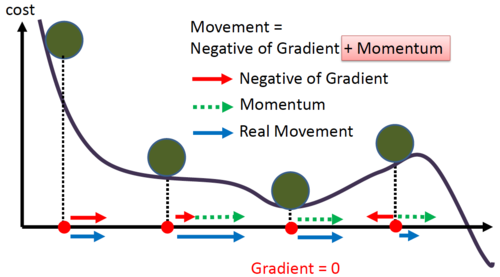
\includegraphics[width = 0.5\textwidth]{figure_man/momentum_illustration_medium.png} \\
	\begin{footnotesize}
	Source: H. Khandewal, \emph{Gradient Descent with Momentum, RMSprop And Adam Optimizer}, Medium 2020. 
	\end{footnotesize}
\end{figure}

\item $\bm{\nu}$ is the (weighted) moving average of the previous gradients:
% \begin{eqnarray*}
%         \bm{\nu}_{i+1} &\leftarrow& \varphi \bm{\nu}_{i} + \underbrace{\nabla_{\bm{\theta}_i} L(y^{(j)}, f_{\bm{\theta}_i}(x^{(j)}))}_{g(\bm{\theta})} \\
%         \bm{\theta}_{i + 1} &\leftarrow&  \bm{\theta}_{i} - \lambda \bm{\nu}_{i+1}
% \end{eqnarray*}
\begin{eqnarray*}
        \bm{\nu}^{[t+1]} &\leftarrow& \varphi \bm{\nu}^{[t]} - \alpha \nabla f(\bm{x}^{[t]}) \\
        \bm{x}^{[t + 1]} &\leftarrow&  \bm{x}^{[t]} + \bm{\nu}^{[t+1]}
\end{eqnarray*}
\item $\alpha$ is the step size and $\varphi \in [0,1]$ is an additional hyperparameter. 
\end{itemize}

\framebreak


\begin{itemize}
% \item Adaptive step size and therefore faster convergence than GD possible.
\item In GD: the step size is simply the gradient multiplied by the learning rate $\alpha$
\item Now, the step size depends on how large and how aligned a sequence of gradients is. The step size grows when many successive gradients point in the same direction.
\item $\varphi$ determines how strongly previous gradients are included in $\bm{\nu}$.
\item Common values for $\varphi$ are 0.5, 0.9 and even 0.99
\item In general, the larger $\varphi$ is relative to the learning rate $\alpha$, the more previous gradients affect the current direction. 
\item $\varphi = 0$ equals gradient descent.
\item Can be seen as GD with \enquote{short term memory} for the direction of motion.
\end{itemize}

\end{vbframe}

%<<eval = FALSE, echo = FALSE>>=
%# generate base data
%options(warn = -1)
%x0 = seq(-3L, 3L, length.out = 200L)
%y0 = cos(x0)
%x1 = x0
%y1 = y0 + rnorm(n = length(y0), sd = 0.3)


%# generate moving average
%ma1 = data.frame(x = x0[(1/(1-0.5)):length(x0)], y = rollapply(y1, FUN = mean, width = (1/(1-0.5))))
%ma1 = rbind(rep(NA, length.out = 2*(200L - length(ma1$x))), ma1)
%ma2 = data.frame(x = x0[(1/(1-0.95)):length(x0)], y = rollapply(y1, FUN = mean, width = (1/(1-0.95) + 1)))
%ma2 = rbind(data.frame(x = rep(NA, length.out = (200L - length(ma2$x))),
%                       y = rep(NA, length.out = (200L - length(ma2$x)))), ma2)
%ma3 = data.frame(x = x0[(1/(1-0.99)):length(x0)], y = rollapply(y1, FUN = mean, width = (1/(1-0.99) + 1)))
%ma3 = rbind(data.frame(x = rep(NA, length.out = (200L - length(ma3$x))),
%                       y = rep(NA, length.out = (200L - length(ma3$x)))), ma3)

%plotdata = data.frame(x0, y0, x1, y1, ma1x = ma1$x, ma1y = ma1$y, ma2x = ma2$x, ma2y = ma2$y,
%                      ma3x = ma3$x, ma3y = ma3$y)

%#plot data and moving average
%plot = ggplot(data = plotdata, aes(x0, y0, color = x))
%plot = plot + geom_line(aes(x0, y0, colour = "cos()"))
%plot = plot + geom_point(aes(x1, y1, colour = "cos() + noise"))
%plot = plot + xlab("x")
%plot = plot + ylab("y")
%plot = plot + xlim(-3, 3)
%plot = plot + scale_colour_manual(values = c("black", "red"))
%plot = plot + theme(legend.position = "bottom")
%plot = plot + theme(legend.title = element_blank())

%plot2 = ggplot(data = plotdata, aes(ma1x, ma1y, color = x))
%plot2 = plot2 + geom_line(aes(ma1x, ma1y, colour = paste('phi', " = 0.5")))
%plot2 = plot2 + geom_line(aes(ma2x, ma2y, colour = paste('phi', " = 0.95")))
%plot2 = plot2 + geom_line(aes(ma3x, ma3y, colour = paste('phi', " = 0.99")))
%plot2 = plot2 + geom_point(aes(x1, y1, colour = "cos() + noise"))
%plot2 = plot2 + xlab("x")
%plot2 = plot2 + ylab("y")
%plot2 = plot2 + xlim(-3, 3)
%plot2 = plot2 + scale_colour_manual(values = c("red", "green", "black", "orange", "yellow"))
%plot2 = plot2 + theme(legend.position = "bottom")
%plot2 = plot2 + theme(legend.title = element_blank())

%grid.arrange(plot, plot2, ncol = 2)

%options(warn = 0)
%@

% \scriptsize
% \begin{itemize}
% \item Kleines $\varphi$ (z.B. $\varphi = 0.5$) führt zu starker Fluktuation .
% \item Großes $\varphi$ (z.B. $\varphi = 0.99$) führt zu guter Glättung jedoch Verschiebung.
% \end{itemize}
% $\rightarrow$ Geringe Richtungsänderung: Erhöhe durch großes $\varphi$ die Geschwindigkeit des Algorithmus.
% \medskip
%
% $\rightarrow$ Starke Richtungsänderung: Verringere durch kleines $\varphi$ die Geschwindigkeit um die Krümmung besser abzubilden.
%
% \framebreak

%\textbf{Connection of velocity, momentum and gradient:}
%
%We consider the momentum in iteration $t$ depending on the previous iterations:
%
%\vspace*{-0.5cm}
%  \begin{eqnarray*}
%    \bm{\nu}^{[t]} &\leftarrow& \varphi \bm{\nu}^{[t-1]} + \nabla f(\bm{x}^{[t]}) \\
%    \bm{\nu}^{[t-1]} &\leftarrow& \varphi \bm{\nu}^{[t-2]} + \nabla f(\bm{x}^{[t-1]}) \\
%    \bm{\nu}^{[t-2]} &\leftarrow& \varphi \bm{\nu}^{[t-3]} + \nabla f(\bm{x}^{[t-2]}) \\
%    \\
%    \bm{\nu}^{[t]} &=& \varphi(\varphi(\varphi \bm{\nu}^{[t-3]} + \nabla f(\bm{x}^{[t-2]})) + \nabla f(\bm{x}^{[t-1]})) + \nabla f(\bm{x}^{[t]})\\
%    \bm{\nu}^{[t]} &=& \varphi^{3} \bm{\nu}^{[t-3]} + \varphi^{2} \nabla f(\bm{x}^{[t-2]}) +\varphi \nabla f(\bm{x}^{[t-1]}) + \nabla f(\bm{x}^{[t]})
%  \end{eqnarray*}
%  \vspace*{-0.6cm}
%\begin{itemize}
%% \item Da $\varphi \in [0,1]$ geht die Funktion $g(\theta_{t-n}), n\in \N$ mit geringerem Gewicht in $\bm{\nu}_{t}$ ein als $g(\theta_{t-(n-1)})$.
%\item Since $\varphi \in [0,1]$, the gradient of the iteration $t-1$ influences the velocity $\bm{\nu}^{[t]}$ more than the gradients of the previous iterations ($t-2, t-3,...$).
%\end{itemize}

%\framebreak

\begin{frame}{Momentum: Example}
	\footnotesize 
	\begin{eqnarray*}
		\bm{\nu}^{[1]} &\leftarrow& \textcolor{blue}{\varphi \bm{\nu}^{[0]} - \alpha \nabla f(\bm{x}^{[0]})} \\[0.1cm]
		\bm{x}^{[1]} &\leftarrow& \bm{x}^{[0]} + \textcolor{blue}{\varphi \bm{\nu}^{[0]} - \alpha \nabla f(\bm{x}^{[0]})} \\[0.1cm]
		\pause
		\bm{\nu}^{[2]} &\leftarrow& \textcolor{red}{\varphi \bm{\nu}^{[1]} - \alpha \nabla f(\bm{x}^{[1]})} \\
		&=& \textcolor{red}{\varphi} \textcolor{blue}{(\varphi \bm{\nu}^{[0]} - \alpha \nabla f(\bm{x}^{[0]}))} - \textcolor{red}{\alpha \nabla f(\bm{x}^{[1]})} \\[0.1cm]
		\bm{x}^{[2]} &\leftarrow& \bm{x}^{[1]} +\textcolor{red}{\varphi} \textcolor{blue}{(\varphi \bm{\nu}^{[0]} - \alpha \nabla f(\bm{x}^{[0]}))} - \textcolor{red}{\alpha \nabla f(\bm{x}^{[1]})} \\[0.1cm]
		\pause
		\bm{\nu}^{[3]} &\leftarrow& \textcolor{green}{\varphi \bm{\nu}^{[2]} - \alpha \nabla f(\bm{x}^{[2]})} \\
		&=& \textcolor{green}{\varphi} (\textcolor{red}{\varphi} \textcolor{blue}{(\varphi \bm{\nu}^{[0]} - \alpha \nabla f(\bm{x}^{[0]}))} - \textcolor{red}{\alpha \nabla f(\bm{x}^{[1]})}) - \textcolor{green}{\alpha \nabla f(\bm{x}^{[2]})} \\[0.1cm]
		\bm{x}^{[3]} &\leftarrow& \bm{x}^{[2]} + \textcolor{green}{\varphi} (\textcolor{red}{\varphi} \textcolor{blue}{(\varphi \bm{\nu}^{[0]} - \alpha \nabla f(\bm{x}^{[0]}))} - \textcolor{red}{\alpha \nabla f(\bm{x}^{[1]})}) - \textcolor{green}{\alpha \nabla f(\bm{x}^{[2]})}  \\
		&=& \bm{x}^{[2]} + \varphi^3\bm{\nu}^{[0]} - \varphi^2\alpha\nabla f(\bm{x}^{[0]}) - \varphi \alpha \nabla f(\bm{x}^{[1]}) - \alpha \nabla f(\bm{x}^{[2]}) \\
		&=& \bm{x}^{[2]} - \alpha(\varphi^2 \nabla f(\bm{x}^{[0]}) + \varphi^1 \nabla f(\bm{x}^{[1]}) + \varphi^0 \nabla f(\bm{x}^{[2]})) + \varphi^3 \bm{\nu}^{[0]} \\
		\pause
		\bm{x}^{[t+1]} &=& \bm{x}^{[t]} - \alpha \displaystyle\sum_{j = 0}^{t} \varphi^j \nabla f(\bm{x}^{[t-j]}) + \varphi^{t+1}\bm{\nu}^{[0]}
	\end{eqnarray*}
	\end{frame}

\begin{vbframe}{Momentum: Example}
	%\framebreak
	Suppose momentum always observes the same gradient $ \nabla f(\bm{x})$:
	\footnotesize 
	\begin{eqnarray*}
		\bm{x}^{[t+1]} &=& \bm{x}^{[t]} - \alpha \displaystyle\sum_{j = 0}^{t} \varphi^j  \nabla f(\bm{x}^{[j]}) + \varphi^{t+1}\bm{\nu}^{[0]} \\
		&=& \bm{x}^{[t]} - \alpha  \nabla f(\bm{x}) \displaystyle\sum_{j = 0}^{t} \varphi^j + \varphi^{t+1}\bm{\nu}^{[0]} \\
		&=& \bm{x}^{[t]} - \alpha  \nabla f(\bm{x}) \frac{1 - \varphi^{t+1}}{1 - \varphi} + \varphi^{t+1} \bm{\nu}^{[0]} \\
		&\to& \bm{x}^{[t]} - \alpha  \nabla f(\bm{x}) \frac{1}{1 - \varphi} \qquad \text{ for } t \to \infty. 
	\end{eqnarray*}
	
	Thus, momentum will accelerate in the direction of $- \nabla f(\bm{x})$ until reaching terminal velocity with step size: 
	$$-\alpha  \nabla f(\bm{x})(1 + \varphi + \varphi^2 + \varphi^3 + ...) = -\alpha  \nabla f(\bm{x}) \frac{1}{1 - \varphi}$$
	E.g. a momentum with $\varphi = 0.9$ corresponds to multiplying the maximum speed by 10 relative to the gradient descent algorithm. 

\framebreak
The vector $\bm{\nu}^{[3]}$ (for $\bm{\nu}^{[0]} = 0$): 
 	\begin{eqnarray*}
 	\bm{\nu}^{[3]} &=& \varphi (\varphi (\varphi \bm{\nu}^{[0]} - \alpha \nabla f(\bm{x}^{[0]})) - \alpha \nabla f(\bm{x}^{[1]})) - \alpha \nabla f(\bm{x}^{[2]}) \\
 	&=& - \varphi^2\alpha\nabla f(\bm{x}^{[0]}) - \varphi \alpha \nabla f(\bm{x}^{[1]}) - \alpha \nabla f(\bm{x}^{[2]})
 	\end{eqnarray*}
 
 \vspace*{-0.2cm}
  \begin{figure}
  \centering
    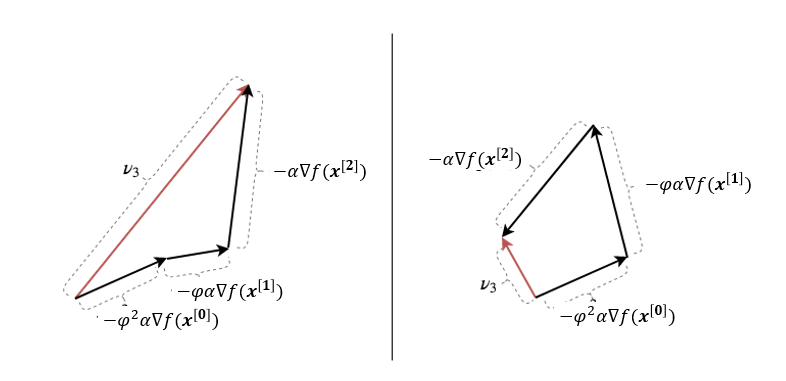
\includegraphics[width = 0.7\textwidth]{figure_man/momentum_vectors.png} \\
    \begin{footnotesize}
    	If consecutive (negative) gradients point mostly in the same direction, the velocity "builds up". On the other hand, if consecutive (negative) gradients point in very different directions, the velocity "dies down". \\
    	Further geometric intuitions as well as a detailed explanation can be found on the following website:
      \url{https://distill.pub/2017/momentum/}
    \end{footnotesize}
  \end{figure}


\end{vbframe}


\begin{vbframe}{GD with momentum: Zig-zagging behavior}

Consider a 2D quadratic form 
$$
	\fx = \xv^\top \bm{C} \xv = \xv^\top \mat{0.5 & 0  \\ 0 & 10} \xv, \quad \xv^\ast = (0, 0)^\top. 
$$ 

Let $\xv^{[0]} = (10, 1)^\top$, and $\alpha = 0.1$. GD shows stronger zig-zagging behavior than GD with momentum. 
\vspace*{-0.2cm}

\begin{center}
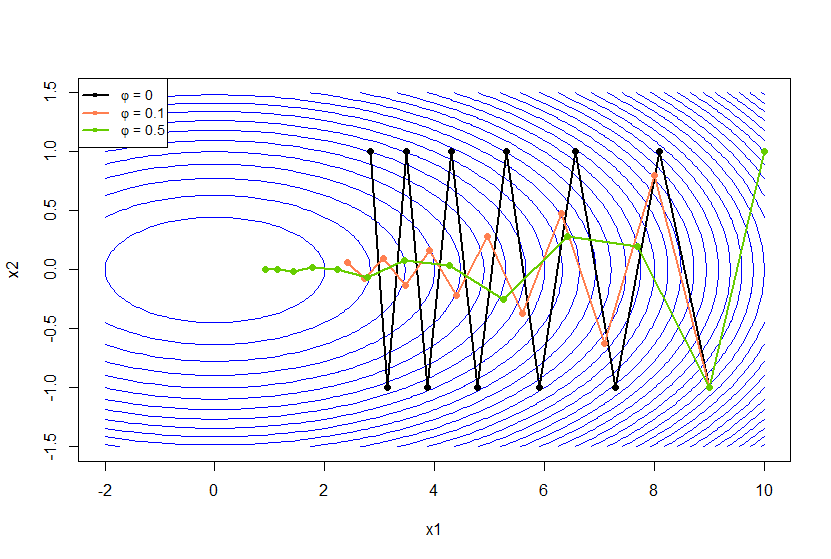
\includegraphics[width = 0.6\textwidth]{figure_man/momentum/compare_gd_momentum.png}
\end{center}

\framebreak
\textbf{Be cautios:} If the momentum is too high, the optimum will probably be missed, rolling past it and back. We might swing back and forth between local optima.
\begin{center}
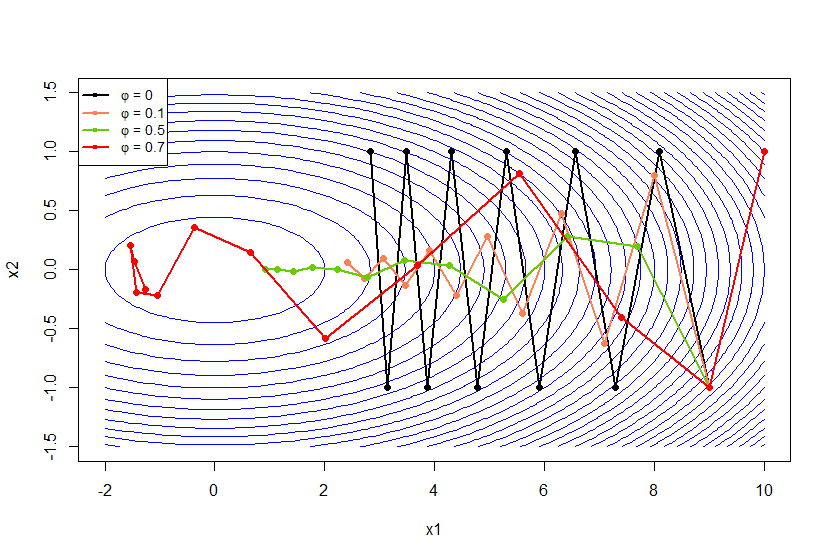
\includegraphics[width = 0.75\textwidth]{figure_man/momentum/comparison_momentum_overshoot.png}
\end{center}

\end{vbframe}


\begin{vbframe}{GD with momentum: Magnitude vanishing}

Consider the 2D quadratic function $f(\bm{x}) = x_{1}^{2} - x_{2}^{2}$with a saddle point at $(0, 0)^\top$. Let $\bm{x}^{[0]} = (-0.5, 0.001)^\intercal$, and $\alpha = 0.1$.

\vspace*{0.3cm}

 The GD is slowing down at the saddle point (vanishing magnitude of the gradient), while GD with momentum \enquote{breaks out} of the saddle point and converges towards the minimum. 

\begin{center}
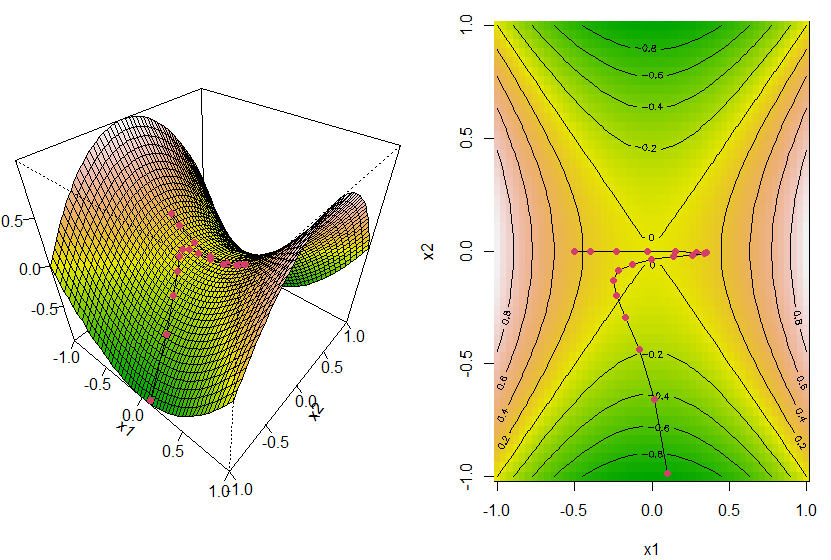
\includegraphics[width = 0.6\textwidth]{figure_man/momentum/sgd_momentum_saddlepoint.png}
\end{center}

%\framebreak
%
%\textbf{Comparison of GD and GD with momentum}
%\medskip
%
%  \begin{figure}
%  \centering
%    \includegraphics[height = 5 cm, width = 9 cm]{figure_man/gd_vs_momentum.png}
%  \end{figure}
%  \vspace*{-0.4cm}
%  \begin{footnotesize}
%  \begin{itemize}
%  \item GD (left) requires many steps and terminates in local minimum.
%  \item Momentum (right) terminates in global minimum.
%  \end{itemize}
%  \end{footnotesize}
\end{vbframe}


\begin{vbframe}{Nesterov's accelerated gradient}
	A slightly modified version is Nesterov momentum with stronger theoretical convergence guarantees for convex functions. Here, the gradient is computed at updated position 
	$$
	\bm{\Tilde{x}} =  \bm{x}^{[t]} + \varphi \bm{\nu}^{[t]}
	$$
	\begin{center}
		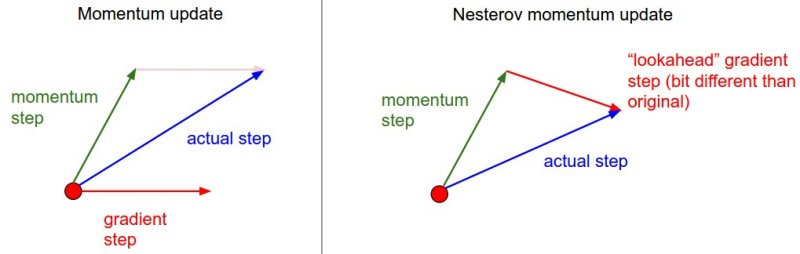
\includegraphics[width = 0.8\textwidth]{figure_man/nesterov.jpeg}
		\footnotesize{Instead of evaluating the gradient at the current position, with Nesterov momentum we evaluate the gradient at the "looked-ahead" position. \\ Source:https://cs231n.github.io/neural-networks-3/}
	\end{center}
\end{vbframe}

\begin{vbframe}{Momentum vs. Nesterov Momentum}
	\begin{figure}
		\vspace{-0.3cm}
		
		\centering
		\scalebox{0.90}{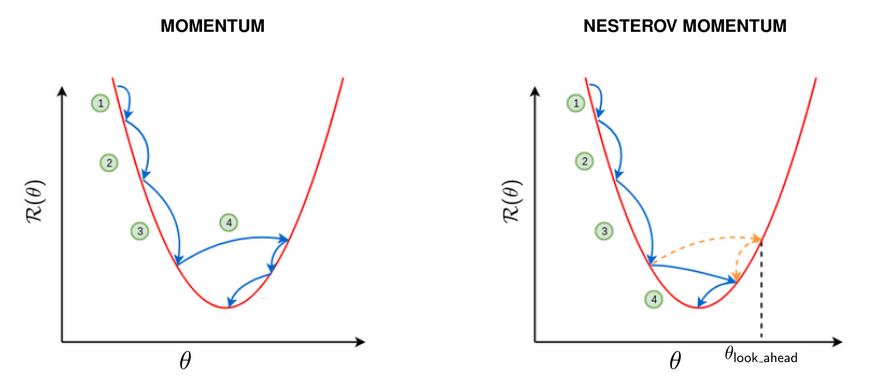
\includegraphics{figure_man/nesterov_momentum.png}}
		\tiny{\\Source: Chandra (2015) \\}
		\footnotesize{Comparison GD with momentum (left) and GD with Nesterov momentum (right) for one parameter $\theta$. The first three updates of $\theta$ are very similar in both cases and the updates become larger due to momentum (accumulation of previous negative gradients). Update 4 is different. In case of momentum, the update overshoots as it makes an even bigger step due to the gradient history. In contrast, Nesterov momentum first evaluates a "look-ahead" point $\theta_{\text{look\_ahead}}$, detects that it overshoots, and slightly reduces the overall magnitude of the fourth update. Thus, Nesterov momentum reduces overshooting and leads to smaller oscillations than momentum. }
	\end{figure}
\end{vbframe}


%%%%%%%%%%%%%%%%%%%%%%%%%%%%%%%%%%%%%%%%%%%%%%%%%%%%%%%%%%%%%%%%%%
%%%%%%%%%%%%%%%%%%%%%%%%%%%%%%%%%%%%%%%%%%%%%%%%%%%%%%%%%%%%%%%%%%

\endlecture
\end{document}

